\documentclass[12pt,a4paper]{article}
\usepackage{cmap} % Makes the PDF copiable. See http://tex.stackexchange.com/a/64198/25761
\usepackage[T1]{fontenc}
\usepackage[brazil]{babel}
\usepackage[utf8]{inputenc}
\usepackage{amsmath}
\usepackage{amsfonts}
\usepackage{amssymb}
\usepackage{amsthm}
\usepackage{textcomp} % \degree
\usepackage{gensymb} % \degree
\usepackage[usenames,svgnames,dvipsnames]{xcolor}
\usepackage{hyperref}
\usepackage{multicol}
\usepackage{graphicx}
\usepackage[margin=2cm]{geometry}
\usepackage{systeme}
\usepackage{icomma}

\hypersetup{
   colorlinks = true,
   allcolors = {blue}
}

% TODO: Consider using exsheets
% http://linorg.usp.br/CTAN/macros/latex/contrib/exsheets/exsheets_en.pdf
%
% http://ctan.org/tex-archive/macros/latex/contrib/exercise/
% Options: answerdelayed,lastexercise,noanswer
\usepackage[answerdelayed,lastexercise]{exercise}

\addto\captionsbrazil{%
\def\listexercisename{Lista de exerc\'icios}%
\def\ExerciseName{Exerc\'icio}%
\def\AnswerName{Solu\c{c}\~ao do exerc\'icio}%
\def\ExerciseListName{Ex.}%
\def\AnswerListName{Solu\c{c}\~ao}%
\def\ExePartName{Parte}%
\def\ArticleOf{de\ }%
}

\renewcommand{\ExerciseHeaderTitle}{(\ExerciseTitle)\ }
\renewcommand{\ExerciseListHeader}{%\ExerciseHeaderDifficulty%
\textbf{%\ExerciseListName\
\ExerciseHeaderNB.\ %
%\ --- \
\ExerciseHeaderTitle}%
%\ExerciseHeaderOrigin
\ignorespaces}
\renewcommand{\AnswerListHeader}{\textbf{\ExerciseHeaderNB.\ (\AnswerListName)\ }}

\renewcommand{\theenumi}{\alph{enumi}}
\renewcommand\labelenumi{(\theenumi) }

\newcommand*\tipo{Prova I}
\newcommand*\turma{CCI192-04U}
\newcommand*\disciplina{ANN0001}
\newcommand*\eu{Helder G. G. de Lima}
\newcommand*\data{11/09/2024}

\author{\eu}
\title{\tipo - \disciplina}
\date{\data}

\begin{document}
\thispagestyle{empty}
\newgeometry{margin=2cm,bottom=0.5cm}
\begin{center}

\includegraphics[width=9.0cm]{marca} \\
\textbf{\tipo\ (\disciplina / \turma)} \\
Prof. \eu\footnote{
Este é um material de acesso livre distribuído sob os termos da licença \href{https://creativecommons.org/licenses/by-sa/4.0/deed.pt_BR}{Creative Commons BY-SA 4.0}}
\end{center}

\noindent Nome do(a) aluno(a): \underline{\hspace{9,7cm}} Data: \underline{\data}

%\section*{Instruções}
\begin{center}\fbox{
\begin{minipage}{14cm}
\begin{footnotesize}
\begin{itemize}
\renewcommand{\theenumi}{\Roman{enumi}}
\item Identifique-se em todas as folhas.
\item Mantenha o celular e os demais equipamentos eletrônicos desligados durante a prova.
\item Justifique cada resposta com cálculos ou argumentos baseados na teoria estudada.
\item Resolva $4$ das $5$ questões (deixe claro que questão não deverá ser corrigida).
\end{itemize}
\end{footnotesize}
\end{minipage}
}
\end{center}

%\section*{Questões}
\begin{ExerciseList}
\Exercise[title={2,5}] Suponha que, ao armazenar a matriz
\(M = \begin{bmatrix}
    \frac{\sqrt{2}}{5} & \frac{1}{5}\\
    \frac{3}{10}        & \frac{\sqrt{2}}{5}
\end{bmatrix}\)
em um computador, as entradas de \(M\) tenham sido truncadas, mantendo apenas três dígitos de suas representações decimais após a vírgula, resultando em uma matriz \(T \approx M\). Calcule o erro percentual ao considerar o determinante de \(T\) como uma aproximação para o determinante de \(M\).
{\color{blue} \textit{(Apresente o resultado final com 6 algarismos após a vírgula)}}

\Answer Como \(\frac{\sqrt{2}}{5} = 0,282842\ldots\), \(\frac{1}{5} = 0,2\) e \(\frac{3}{10} = 0,3\), temos
\(T = \begin{bmatrix}
    0,282 & 0,2\\
    0,3   & 0,282
\end{bmatrix}\).
Assim, calculamos
\[
\det(T) = 0,282 \cdot 0,282 - 0,2 \cdot 0,3 = 0,079524 - 0,06 = 0,019524.
\]
Por outro lado, o determinante de \(M\) é dado por
\[
\det(M) = \frac{\sqrt{2}}{5} \cdot \frac{\sqrt{2}}{5} - \frac{1}{5} \cdot \frac{3}{10} = \frac{2}{25} - \frac{3}{50} = \frac{1}{50} = 0,02.
\]

Portanto, o erro percentual é
\[
\varepsilon_{per} = \left|\frac{0,019524 - 0,02}{0,02}\right| \times 100\% = \left|\frac{-0,000476}{0,02}\right| \times 100\% = 2,38\%.
\]


\Exercise[title={2,5}] Seja \(f(x) = \tan(\ln(x))\). Verifique que o método da \textbf{posição falsa} pode ser aplicado usando o intervalo inicial \([a_0, b_0] = [15, 78]\) e obtenha uma aproximação \(x_k\) do zero da função \(f(x)\) tal que \(|f(x_k)| \leq 0,01\). {\color{blue} \textit{(Certifique-se de que a calculadora esteja configurada para usar radianos, e arredonde os valores obtidos com 4 algarismos após a vírgula)}}

\Answer Considerando que \(f(15) = -0,4629 < 0 < 2,6919 = f(78)\) e que a função \(f\) é contínua em \([15, 78]\), o teorema de Bolzano garante a existência de um zero de \(f\) nesse intervalo, conforme pode ser confirmado na figura a seguir:

\begin{center}
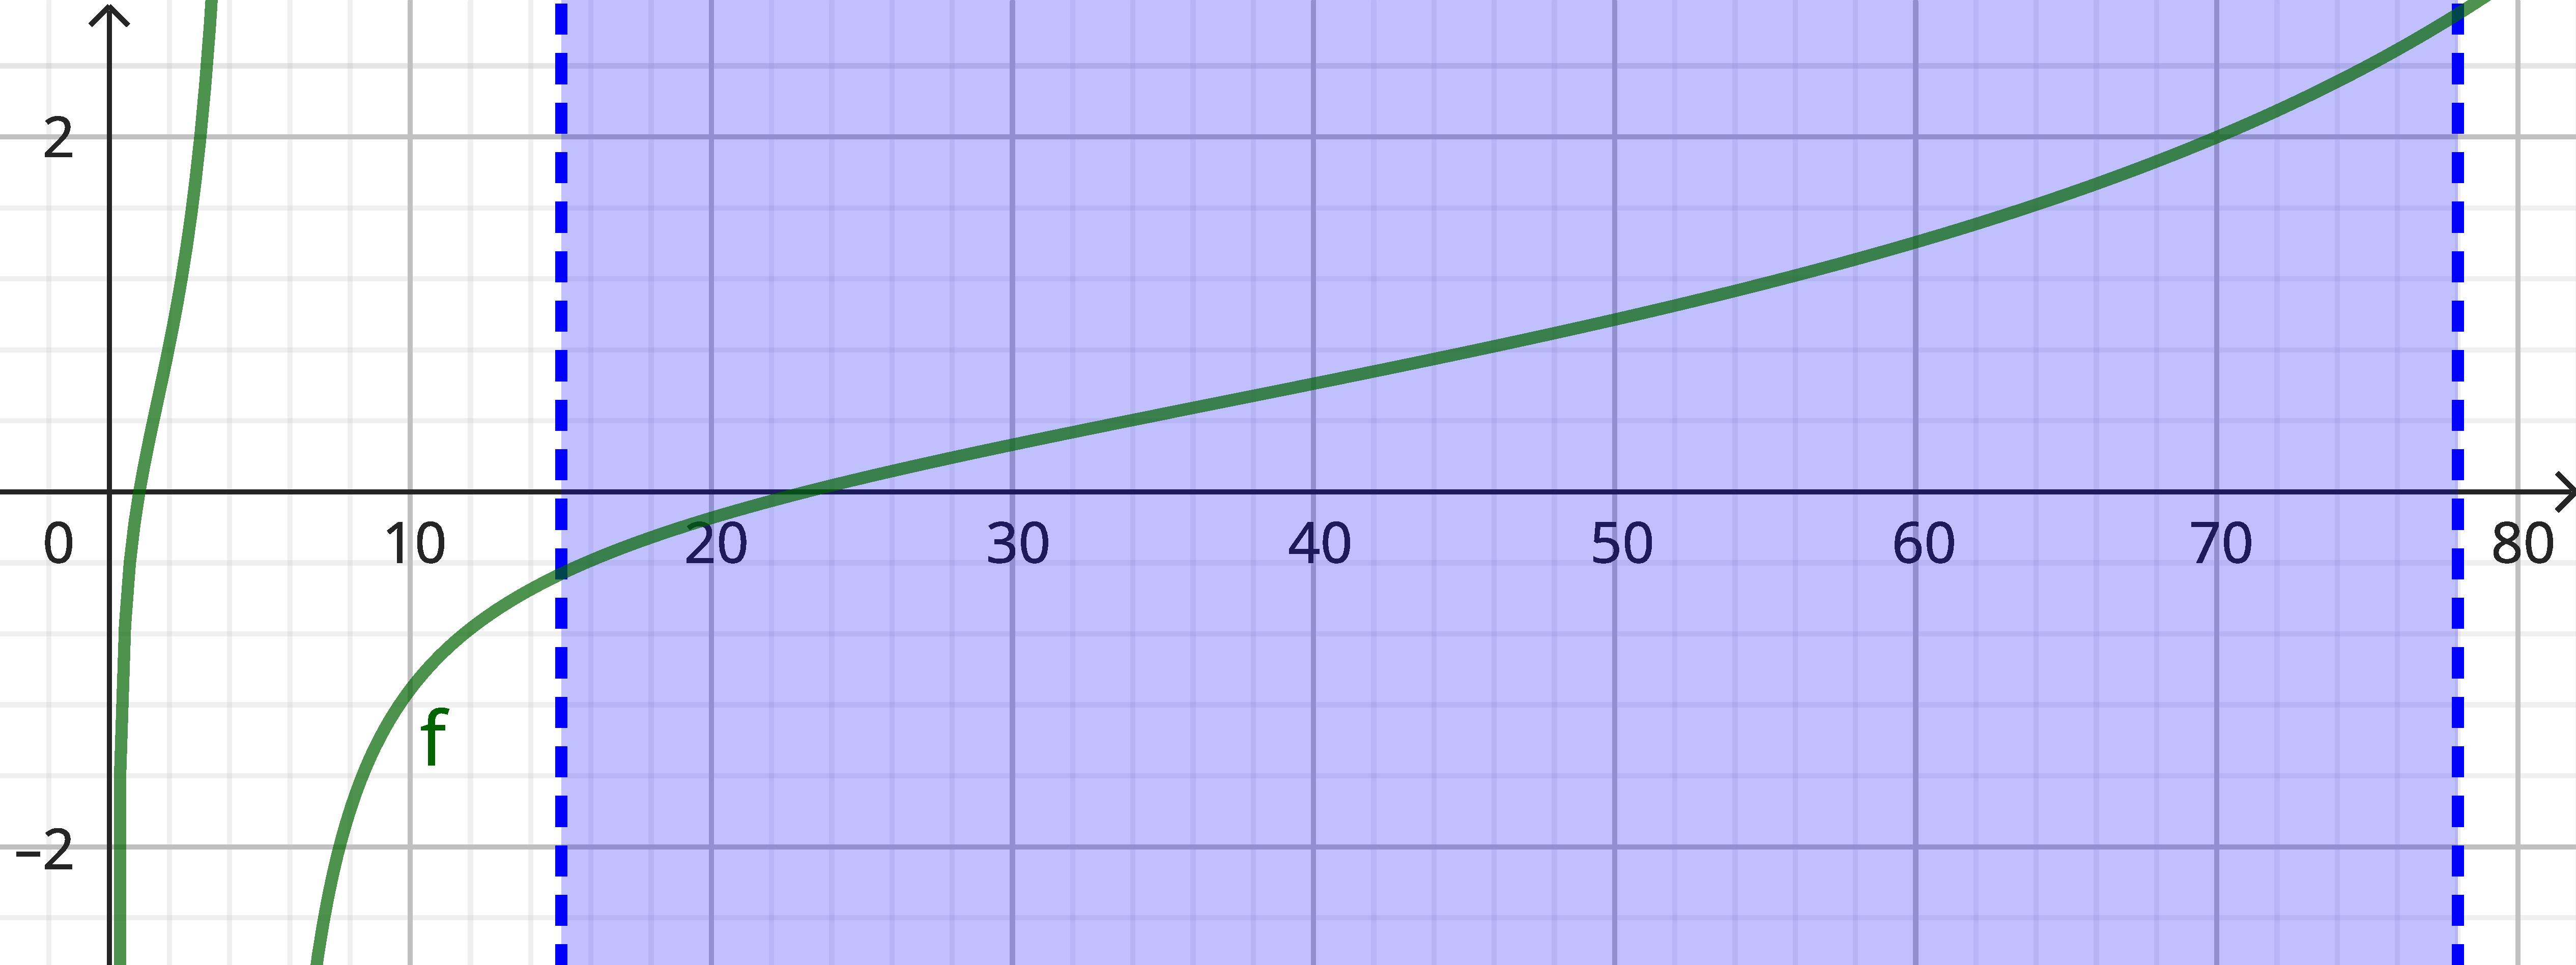
\includegraphics[width=0.5\textwidth]{img/posição-falsa.pdf}
\end{center}

Com as condições anteriores, assegura-se que a sequência \((x_k)_{k=0}^\infty\) gerada pelo método da posição falsa será convergente. Os primeiros termos dessa sequência são obtidos conforme segue (com arredondamento na quarta casa decimal a cada iteração):
\medskip
\begin{center}
\begin{tabular}{rrrrrrrc}
\hline
$k$ & $a_k$ & $x_k$ & $b_k$ & $f(a_k)$ & $f(x_k)$ & $f(b_k)$ & $f(a_k) \cdot f(x_k)$ \\
\hline
0 & 15 & 24,2439 & 78 & -0,4629 & 0,0466 & 2,6919 & < 0 \\
1 & 15 & 23,3984 & 24,2439 & -0,4629 & 0,0111 & 0,0466 & < 0 \\
2 & 15 & 23,2017 & 23,3984 & -0,4629 & \textbf{0,0026} & 0,0111 & < 0 \\
\hline
\end{tabular}
\end{center}
\medskip
Como \(|f(x_2)| = 0,0026 < 0,01\) (após arredondar na quarta casa decimal), concluímos que a aproximação \(x_2 = 23,2017\) da raiz de \(f\) atende à precisão desejada.

\Exercise[title={2,5}] Seja \(f:\mathbb{R} \to \mathbb{R}\) definida por \(f(x) = e^{-x} - x\) e considere a equação \(f(x) = 0\).
\begin{enumerate}
    \item Obtenha uma função de iteração \(\varphi(x)\) para a qual seja possível demonstrar, por meio de argumentos teóricos, que se \(x_0 = \frac{3}{5}\) e \(x_k = \varphi(x_{k-1})\) para \(k \in \mathbb{N}\), então a sequência \((x_k)_{k \in \mathbb{N}}\) converge para algum \(\overline{x}\) tal que \(f(\overline{x}) = 0\). Apresente todos os detalhes dessa argumentação.
    \item Utilize a função de iteração obtida para calcular, pelo método da \textbf{iteração de ponto fixo}, uma aproximação \(x_k \approx \overline{x}\) cujo erro relativo estimado por \(\varepsilon_{\text{rel}} \approx \dfrac{|x_k - x_{k-1}|}{|x_k|}\) satisfaça \(|\varepsilon_{\text{rel}}| \leq 0,03\). {\color{blue} \textit{(Arredonde os valores obtidos com 4 algarismos após a vírgula)}}
\end{enumerate}
\Answer \begin{enumerate}
\item Como a equação \(f(x) = e^{-x} - x = 0\) equivale a \(x = e^{-x}\), a função \(\varphi(x) = e^{-x}\) é uma função de iteração para \(f\). Além disso, temos \(\varphi^\prime(x) = -e^{-x}\) e as funções \(\varphi\) e \(\varphi^\prime\) são contínuas em \(\mathbb{R}\). Considerando que \( |\varphi^\prime(x)| = \left|-e^{-x}\right| = e^{-x} = \frac{1}{e^x} \), temos
\[
|\varphi^\prime(x)| < 1
\Leftrightarrow
\frac{1}{e^x} < 1
\Leftrightarrow
1 < e^x
\Leftrightarrow
x \in (0, +\infty).
\]
Além disso, \(f\) é uma função contínua tal que \(f\left(\frac{1}{2}\right) \approx 0,1065 > 0\) e \(f(1) \approx -0,6321 < 0\). Portanto, pelo teorema de Bolzano, existe \(\overline{x} \in \left(\frac{1}{2}, 1\right)\) tal que \(f(\overline{x}) = 0\). Em particular, se \(I\) for um intervalo centrado em \(\overline{x}\), ou seja, \(I = \left(\overline{x}-\delta, \overline{x}+\delta\right)\), com raio \(\delta < \frac{1}{2}\), então \(I \subset (0, +\infty)\) e pode-se obter \(\overline{x}\) pelo método de iteração de ponto fixo como o limite da sequência dada por \(x_k = \varphi(x_{k-1})\), para qualquer \(x_0 \in I\), incluindo \(x_0 = \frac{3}{5} = 0,6\).

\item Os primeiros termos dessa sequência são os seguintes (arredondados na quarta casa decimal a cada iteração):

\begin{center}
\begin{tabular}{cccc}
\hline
$k$ & $x_k$ & $\varphi(x_k)$ & $\varepsilon_{\text{rel}}(x_k)$\\
\hline
0 & 0,6000 & 0,5488 & - \\
1 & 0,5488 & 0,5776 & 0,0933 \\
2 & 0,5776 & 0,5612 & 0,0499 \\
3 & 0,5612 & -      & \textbf{0,0292} \\
\hline
\end{tabular}
\end{center}
Portanto um valor aproximado de $\overline{x}$ nas condições exigidas é $x_3 = 0,5612$, que tem um erro relativo aproximado inferior a $0,03$.
\end{enumerate}\Exercise[title={2,5}] Mostre que, apesar da função \(f(x) = x^3 - 2x + 2\) ter um zero no intervalo \([-2, 2]\), não é possível usar a aproximação inicial \(x_0 = 0\) para obtê-lo pelo método de \textbf{Newton-Raphson}. Interprete geometricamente.

\Answer A função \(f\) é contínua, e \(f(-2) = -2 < 0 < 6 = f(2)\), logo há um zero no intervalo \((-2, 2)\). Como \(f^\prime(x) = 3x^2 - 2\), as iterações do método de Newton-Raphson são obtidas pela equação:
\[
x_k = x_{k-1} - \frac{x_{k-1}^3 - 2x_{k-1} + 2}{3x_{k-1}^2 - 2}.
\]
Assim, se \(x_0 = 0\), temos:
\[
x_1 = 0 - \frac{0^3 - 2 \cdot 0 + 2}{3 \cdot 0^2 - 2} = 1,
\]
e
\[
x_2 = 1 - \frac{1^3 - 2 \cdot 1 + 2}{3 \cdot 1^2 - 2} = 0.
\]
Portanto, a sequência resultante será \((x_k)_{k=0}^\infty = (0, 1, 0, 1, 0, \ldots)\), que não converge.

Geometricamente, o que ocorre é que a aproximação inicial \(x_0 = 0\) não está suficientemente próxima do verdadeiro zero de \(f\). A interseção da reta tangente ao gráfico de \(f\) em \((0, f(0))\) com o eixo \(x\) gera uma aproximação \(x_1\) que é pior do que a inicial. A partir de \(x_1\), a reta tangente em \((1, f(1))\) intersecta o eixo \(x\) novamente na aproximação inicial \(x_0\), resultando em uma sequência que alterna periodicamente entre \(x_0\) e \(x_1\).

\begin{center}
    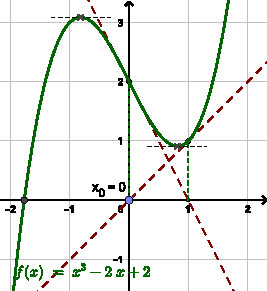
\includegraphics[width=5cm]{img/newton-raphson.pdf}
\end{center}

Do ponto de vista teórico, ao observar que \(f\) tem pontos críticos em \(x = \pm\sqrt{\frac{2}{3}}\), onde \(f^\prime(x) = 0\), conclui-se que \(m = \min_{x \in [-2, 2]} |f^\prime(x)| = 0\), o que impede a aplicação do teorema que forneceria uma condição suficiente para a convergência do método de Newton-Raphson.


\Exercise[title={2,5}] A função \(f(x) = x + \ln(x)\) possui um único zero \(\overline{x} > 0\). Calcule uma aproximação \(x_k \approx \overline{x}\) que satisfaça \( |f(x_k)| \leq 0,01 \) e \( |x_k - x_{k-1}| \leq 0,01 \) usando o método da \textbf{secante}, com aproximações iniciais \(x_{-1} = 0,3\) e \(x_0 = 0,9\).

{\color{blue} \textit{(Arredonde os valores obtidos com 4 dígitos após a vírgula)}}

\Answer Os termos da sequência \((x_k)_{k=0}^\infty\) gerada pelo método da secante são obtidos pela fórmula
\[
x_k = \dfrac{x_{k-2}f(x_{k-1}) - x_{k-1}f(x_{k-2})}{f(x_{k-1}) - f(x_{k-2})},
\]
considerando \(x_{-1} = 0,3\) e \(x_0 = 0,9\). Os primeiros termos são calculados como segue (com arredondamento no quarto dígito decimal a cada iteração):
\medskip
\begin{center}
\begin{tabular}{rrrrrrrc}
\hline
$k$ & $x_{k-2}$ & $x_{k-1}$ & $x_k$ & $f(x_{k-2})$ & $f(x_{k-1})$ & $f(x_k)$ & $|x_k - x_{k-1}|$ \\
\hline
1 & 0,3000 & 0,9000 & 0,6193 & -0,9040 & 0,7946 & 0,1401 & 0,2807 \\
2 & 0,9000 & 0,6193 & 0,5592 & 0,7946 & 0,1401 & -0,0220 & 0,0601 \\
3 & 0,6193 & 0,5592 & 0,5674 & 0,1401 & -0,0220 & \textbf{0,0007} & \textbf{0,0082} \\
\hline
\end{tabular}
\end{center}
\medskip
Como \( |f(x_3)| = 0,0007 < 0,01 \) e, além disso, \( |x_3 - x_2| = 0,0082 \leq 0,01 \), conclui-se que a aproximação \(x_3 = 0,5674\) para o zero de \(f\) atende à precisão requerida.

\textbf{Observação}: Note que \(x_2 = 0,5592\) foi calculado a partir de \(x_1 = 0,6193\) e \(x_0 = 0,9\), e não de \(x_{-1} = 0,3\). Isso ocorre porque o método da secante utiliza as duas aproximações mais recentes, em vez de considerar as duas últimas em que ocorre troca de sinal de \(f\), como seria o caso no método da posição falsa.
\end{ExerciseList}

\vfill
\begin{center}
BOA PROVA!
\end{center}

\newpage
\restoregeometry
\section*{Respostas}
\shipoutAnswer
\end{document}
